\documentclass{article}
\usepackage[landscape]{geometry}
\usepackage[utf8]{inputenc}
\usepackage[T2A]{fontenc}
\usepackage[russian]{babel}
\pagestyle{empty}
\usepackage{microtype}
\usepackage{graphicx}
\usepackage{makecell}
\usepackage{xcolor}
\usepackage{dejavu}
\usepackage{hyperref}
  \hypersetup{colorlinks=true,allcolors=blue!40!black}
\begin{document}
\def\zoldversion{0.2.4}

\pagecolor{white}
\newcommand\slide[1]{%
  \pagebreak\topskip0pt\vspace*{\fill}%
  \begin{center}\huge%
  #1
  \end{center}%
  \vspace*{\fill}%
}

\slide{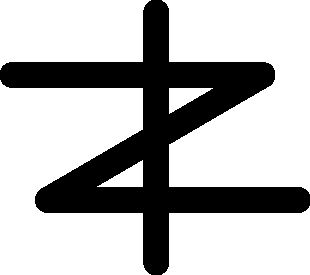
\includegraphics[scale=1]{../images/zerocracy-logo.pdf}\\
Zerocracy, Inc.\\[1em]
\large Palo Alto, CA\\
\large \href{https://www.zerocracy.com}{www.zerocracy.com}}

\slide{Согласно множеству исследований%
\footnote{%
  \href{https://www.projectsmart.co.uk/white-papers/chaos-report.pdf}{Chaos Report} (2015) by Standish Group.
}
большинство проектов по разработке программного обеспечения
в той или иной степени терпят неудачу --- срывают сроки, перерасходуют бюджет, не реализуют
ожидаемый функционал или отстают в качестве. Интересно то, что недостаточная техническая компетенция команды лишь изредка является
причиной провалов. В подавляющем большинстве ошибок виноваты менеджеры,%
\footnote{%
  \href{https://www.infoq.com/articles/software-failure-reasons}{The Most Common Reasons Why Software Projects Fail} (2015) at InfoQ.
}
которые упускают
важную информацию, неверно оценивают объемы работ, стоимость и сроки, или забывают обновить
планы.}

\slide{При современном уровне развития технологий, на службу менеджерам можно и нужно поставить
искусственный интеллект, который, общаясь с программистами в интерактивном режиме,
поможет регулярно и четко выполнять множество рутинных операций, необходимых
любому проекту --- от составления планов-графиков, распределения задач между людьми,
контроля результата, оплаты работы и оценки качества до принятия решений
об индивидульных компетенциях каждого программиста, а затем их найма, увольнения
и перерасчета тарифов оплаты.}

\slide{Идея усилить менеджеров искусственным интеллектом родилась в 2009-м году.
Первая версия была создана в 2010-м, а годом позже была подана заявка
\href{https://patents.google.com/patent/US20110196798}{US 12/703,202} в патентное ведомство США.
В 2013-м году была создана вторая версия,
которая устраняла недостатки первой, однако и она оказалась недостаточно
эффективной. Год спустя, в 2014-м мы разработали и запустили третью версию,
которая наконец доказала работоспособность идеи. За два последующих года через нее
прошло более 250 программистов, 25 проектов и было написано более 400 тысяч
строк кода.}

\slide{В 2016-м году была начата разработка четвертой версии, на создание
которой было потрачено полтора года. Она была выпущена на рынок в марте 2018
и к настоящему моменту успешно управляет несколькими проектами и более чем сотней
программистов.
Всего в проект к настоящему моменту было инвестировано около миллиона долларов
и более восьми лет работы и экспериментов.
Подробнее о команде проекта и нашей глобальной миссии можно прочитать
в \href{https://papers.zold.io/zerocracy-deck.pdf}{Zerocracy Deck}.}

\slide{%
Главным идеологом и владельцем проекта является \href{https://www.yegor256.com/about-me.html}{Егор Буга\'{е}нко},
предприниматель и программист с многолетним стажем;
автор нескольких книг по объектно-ориентированному программированию,%
\footnote{%
  Большинство книг публикуются и продаются компанией
  \href{https://www.amazon.com/Yegor-Bugayenko/e/B01AM1QMDK/}{Amazon}:
  Elegant Objects (\href{http://goo.gl/W2WVMk}{том 1} и \href{http://amzn.to/2pD42k3}{том 2}),
  \href{https://amzn.to/2u9BbqF}{Code Ahead},
  \href{https://goo.gl/DUcXm9}{256 Bloghacks}.
}
в том числе на русском языке%
\footnote{%
  Elegant Objects \href{https://www.piter.com/collection/all/product/elegantnye-obekty-java-edition}{была издана}
  издательством Питер на русском языке в 2018-м году.
};
\href{https://www.yegor256.com/talks.html}{докладчик} на многих международных IT конференциях;
\href{https://github.com/yegor256}{создатель и архитектор} ряда программных продуктов и библиотек с открытым кодом;
венчурный инвестор в \href{https://www.seedramp.com}{SeedRamp}.\\[1em]

{\normalsize\begin{tabular}{cccccc}
  \makecell{
  
\includegraphics[height=6em]{../images/yegor-bugayenko.jpg}\\
  CEO и основатель\\
  \textls[-10]{\href{https://www.yegor256.com/about-me.html}{Yegor Bugayenko}}}
&
  \makecell{%
  
\includegraphics[height=6em]{../images/kiril-cherniavsky.jpg}\\
  Архитектор\\
  \textls[-10]{\href{https://github.com/g4s8}{Kiril Cherniavsky}}}
&
  \makecell{%
  
\includegraphics[height=6em]{../images/erik-larson.jpg}\\
  Советник\\
  \textls[-10]{\href{https://www.linkedin.com/in/erik-larson-b287ba9/}{Erik J. Larson}}}
&
  \makecell{%
  
\includegraphics[height=6em]{../images/carlos-miranda.jpg}\\
  Разработчик\\
  \textls[-10]{\href{https://github.com/carlosmiranda}{Carlos Miranda}}}
&
  \makecell{%
  
\includegraphics[height=6em]{../images/krzysztof-krason.jpg}\\
  Разработчик\\
  \textls[-10]{\href{https://github.com/krzyk}{Krzysztof Kraso\'n}}}
&
  \makecell{%
  
\includegraphics[height=6em]{../images/george-aristy.jpg}\\
  Разработчик\\
  \textls[-10]{\href{https://github.com/llorllale}{George Aristy}}}
\end{tabular}}%
}

\slide{Клиентами Zerocracy потенциально являются все компании, которым необходимо
разрабатывать программные продукты и которые недовольны существующим положением
вещей --- их проекты терпят неудачи, а программисты плохо мотивированны
работать на результат. При работе с Zerocracy клиент получает: 1) прогнозируемость
результатов как по срокам, так и по затратам, 2) существенное
снижение затрат, 3) резкое повышение мотивации персонала, а также 4) рост
качества программного продукта.}

\slide{По нашей информации, Zerocracy является
единственным продуктом в индустрии, который настолько радикально изменяет
формат взаимодействия участников проектов по разработке программного обеспечения.%
\footnote{%
  Рекомендуем посмотреть доклад
  \href{https://www.youtube.com/watch?v=7EytYc7K5JA}{eXtremely Distributed Software Development}
  нашего CEO Егора Бугаенко на конференции DevTernity в Риге в 2016-м году.
}
Уникальность и одновременно беспрецедентная эффективность наших технологий и методологии
обеспечивают Zerocracy высокую инвестиционную привлекательность.}

\slide{Доходность проекта напрямую зависит от количества активно
работающих программистов. Главная трудность их привлечения состоит в том, что наша методология
управления сильно отличается от тех, к которым
привыкли программисты, работающие в офисах: в офисах
они получают оплату за календарный месяц, проведенный в проекте, а у нас
--- за выполненные микрозадачи. Для того, чтобы найти программиста на рынке,
убедить его работать с нами и провести тренинги, уходит
около двух месяцев и \$3,000.}

\slide{Каждый активно работающий программист приносит около \$1,200 дохода
в месяц. Таким образом, при правильной комбинации рекламы, продаж и подбора
программистов, на каждый \$100K вложенных средств, Zerocracy потенциально способна
создавать доход в размере около \$40K в месяц.
В настоящий момент проекту требуются инвестиции в размере \$1.6M, которые
будут потрачены на привлечение программистов, маркетинг и продажи, а также
на развитие нашего уникального платежного инструмента --- криптовалюты \href{https://www.zold.io}{Zold}.
Более подробные цифры можно найти в \href{https://papers.zold.io/executive-summary.pdf}{Executive Summary}.}

\slide{%
  \Large 555 Bryant Str, Ste 470\\
  \Large Palo Alto, CA 94301\\
  \Large 408.692.4742\\
  \Large \href{mailto:team@zerocracy.com}{team@zerocracy.com}\\[1em]
  \normalsize\texttt{\zoldversion\qquad\today}}

\end{document}
